\chapter{Solution} To build an effective and easy to use hand gesture recognition system for NAO, various tools and technologies were studied during this thesis. Figure \ref{fg:hri:components} shows the individual components which are essential part of this thesis in implementing the goal. The main challenge is to find a solution that can integrate all these components into a robust system. However, due to the computational and compatibility limitations of NAO, we have faced problems in implementing few contemplated solutions which are described in the next section. Finally, the successful solution in achieving the goal will be discussed in the following sections.

\begin{figure}
	[h] \centering 
	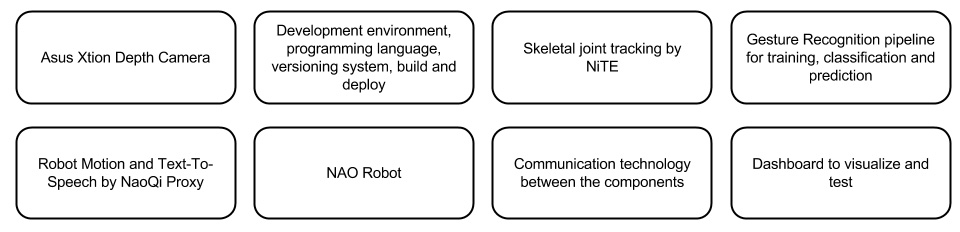
\includegraphics[height=35mm]{figures/content/hri-components.jpg} \caption{Component} \label{fg:hri:components} 
\end{figure}


\section{Experimental Designs} 
\subsection{Everything On-Board} First experiment design was conceived in a way that depth camera, skeletal joint tracking, gesture recognition infrastructure and robot motion will be embedded into the on-board computer of NAO. However, gesture recognition infrastructure is composed of computationally intensive machine learning processes and along with skeletal joint tracking by NiTE had pushed NAO to 100 $ \% $ CPU load consistently. --- Show htop of NiTE cpu consumption ----

\subsection{Extending NAO with Single Board Computer} In order to escape the computational limitation of NAO, another experimental design was contemplated, that the robot will be extended as shown in the figure \ref{fg:nao:bag} with a powerful Single Board Computer such as pcDuino or RaspberryPi. However, Asus Xtions higher power consumption of 2.5 Watts with weight of 250 grams, pcDuinos power consumption of 2A at 5VDC with weight of 100 grams and additional weight by 3D printed mounts, heat sinks and wires will make NAO to be heavier and ultimately result in poor motion performances and higher power consumption. 

\begin{figure}
	[h] \centering 
	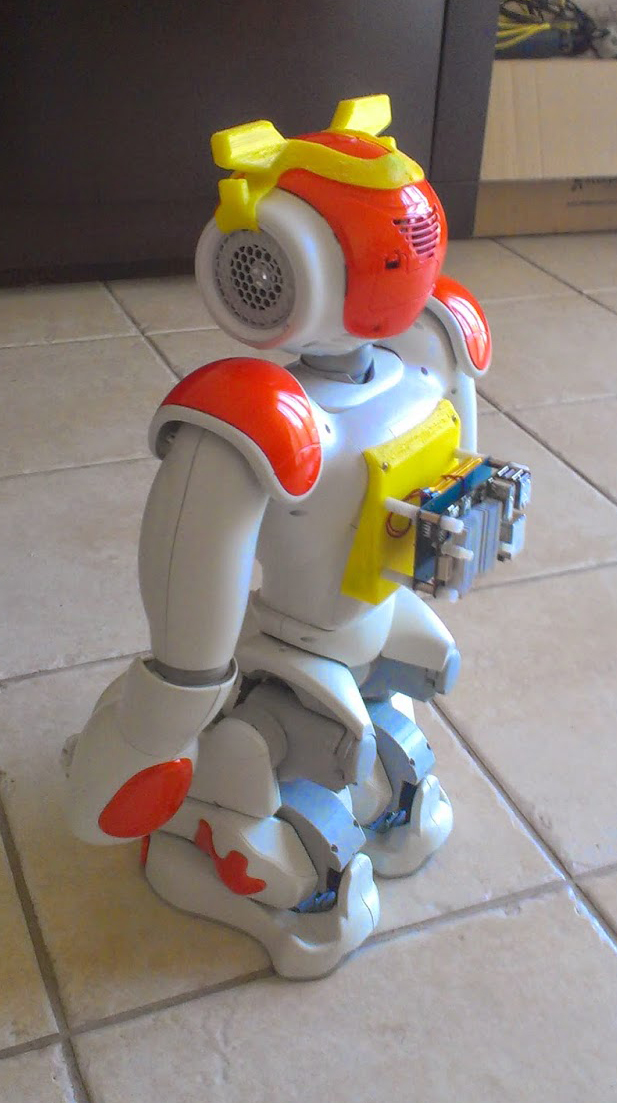
\includegraphics[height=7cm]{figures/content/nao-bag.jpg} \caption{3D printed mount to extend NAO with an external Single Board Computer. \cite{19} } \label{fg:nao:bag} 
\end{figure}


\subsection{Everything Off-Board} This experimental design pushes all the components to an off-board computer that could be a PC connected with depth camera at a fixed location. User will gesticulate in front of the camera and all processing will be done on PC. Finally predicted gesture will be transformed into a motion and voice, and it will be sent to NAO via Aldebaran proxies using WLAN. This design completely decouples the robot from other components and degrades the natural interaction between human and the robot. However, this design will suit for other applications such as indoor navigation and localization of NAO.

\section{Architecture } After analyzing the disadvantages of other experimental designs, the final design was chosen to build an efficient real-time hand gesture recognition for human-robot interaction using skeletal points. Figure \ref{fg:hri:architecture} shows the architecture of the solution that was implemented during this thesis by grouping many components into 4 different modules which serve various purposes. Each module is implemented in different environment as shown in the figure and they communicate with one another to complete the data flow. All these modules uses a common configuration file that contains information such as port number, host name and log path.

\begin{figure}
	[h] \centering 
	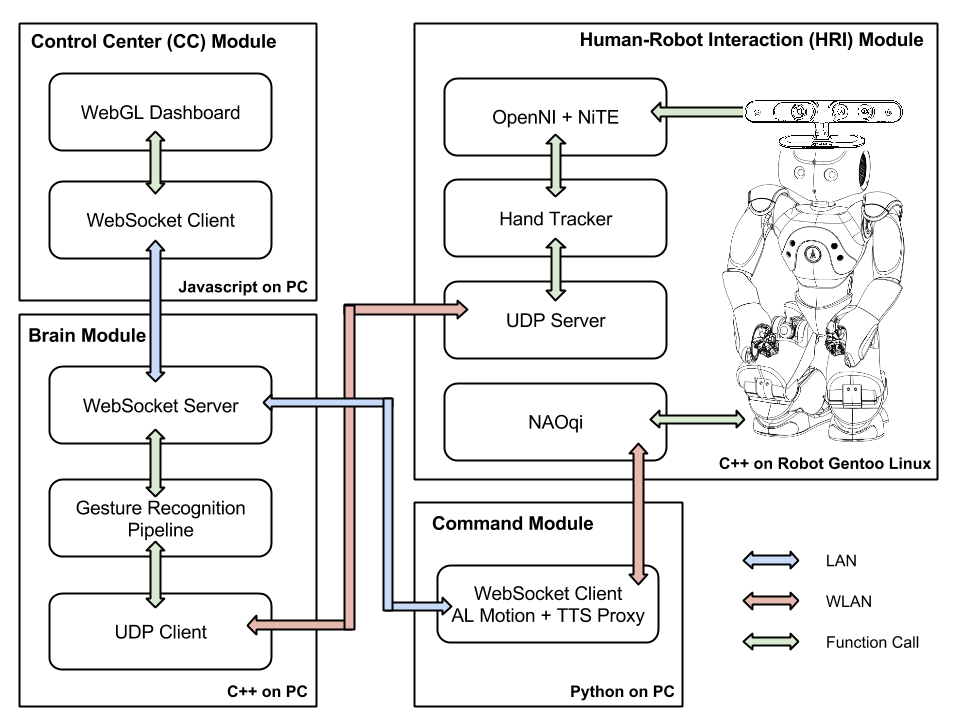
\includegraphics[height=11cm]{figures/content/hri-architecture.png} \caption{HRI Architecture} \label{fg:hri:architecture} 
\end{figure}


\subsection{Human-Robot Interaction (HRI) Module} HRI is the main module that is implemented first in order to get the raw data from the depth sensor and process it to track the skeletal joint positions in real world coordinates. This module is deployed on the general purpose computer that is running inside the robot with necessary libraries and drivers. Especially OpenNI library needs depth camera driver and NiTE library needs its training data.

HRI module is composed of 3 components which are UDP Server, Gesture tracker and Skeleton tracker. They are developed in C++ using a core library called Boost and NiTE 2 framework is used for the purpose of skeletal joints tracking.

Boost is a set of libraries for the C++ programming language that provide support for tasks and structures such as linear algebra, pseudo random number generation, multi threading, image processing, regular expressions, and unit testing. It contains over eighty individual libraries.

This module requests the user to select Gesture tracker or Skeleton tracker, when the program is started. Depending on the selection, it creates 2 threads, one for the UDP server and one for the NiTE tracker. NiTE tracker waits for a new frame from the depth camera till some key was pressed to interrupt the loop, exiting the thread and finally close the program. 

\subsubsection{UDP Server}
HRI module has to process the raw information from the depth camera and it has to send it to Brain module for the purpose of gesture recognition. As show in the architecture diagram \ref{fg:hri:architecture}, Brain module must be connected via Wireless Local Area Network (WLAN). WLAN at 2.4GHz readily is available on NAO and lead us to a solution, where we have to choose an UDP protocol to transmit the processed data from depth camera. UDP was chosen over other protocols because depth camera produces 30 depth images per second and transferring such a large amount of data using conventional communication technologies such as TCP will be create much overhead and delay in the communication.

Due to asynchronous requirement of the server, Boost Asio library is used to implement UDP server. Boost.Asio is a cross-platform C++ library for network and low-level I/O programming that provides developers with a consistent asynchronous model using a modern C++ approach.

UDP Server is basically an asynchronous programs that creates an UDP socket and listens to an port on the local machine. In this case, we have created a common configuration file that contains port numbers for each module in this project. Therefore, this server listens to the 5005 on NAO and waiting for the clients to connect. 

Once the client is connected, it stores the endpoint details of the client such as IP address and the port number of the UDP client (Brain module), so that it can communicate with the Brain module whenever there is some data to be transmitted. Asynchronous functionality Boost.Asio calls the callback handler only when there is communication with the clients and waits in the thread for the next communication.

\subsubsection{Gesture Tracker}
Gesture tracker is a component of HRI module that makes use of NiTE framework to localize the hand of user in the field of view and track the hand position till the hand leaves the field of view (FOV) or hand is touching another object or hidden by an object. 

It uses HandTracker class of NiTE framework and it needs to go through following steps before it can track a hand.

\begin{itemize}
	\item NiTE framework must be initialized using NiTE::initialize() function.
	\item Depth camera must be connected and hand tracker must be created using OpenNI compatible  device id. If not, default depth camera will be selected.
	\item NiTE Gestures such as Wave or Click detection must be initiated in order to localize the hand at first.
	\item NiTE::HandTrackerFrameRef must be read continuously for a new depth image frame.
	\item If Wave or Click gesture is detected, then hand tracking will be started using the position of hand that triggered the gesture.
\end{itemize}

Once the hand is been tracked, the hand will be added an id and it will be added to HandTrackerFrameRef. NiTE framework allow users to add many number of hand and it will be tracked till there is enough computation power  and hands are not overlapping. HandTrackerFrameRef contains the array of all active hands and every hand is an object of NiTE::HandData. It contains the position of the hand in 3 dimensional float stored in a class called Point3f.


However, functionalities gesture tracker are not only  to track hand, but also send these information to Brain module via UDP. Therefore, C++  NiTE::HandData objects must be serialized before transmitted over the network.

 

\subsection{Brain Module}

\subsection{Control Center (CC) Module}

\subsection{Command Module} 
